\documentclass[
    12pt, % Schriftgröße
    DIV10,
    ngerman, % für Umlaute, Silbentrennung etc.
    a4paper, % Papierformat
    oneside, % einseitiges Dokument
    titlepage, % es wird eine Titelseite verwendet
    parskip=half, % Abstand zwischen Absätzen (halbe Zeile)
    headings=normal, % Größe der Überschriften verkleinern
    listof=totoc, % Verzeichnisse im Inhaltsverzeichnis aufführen
    bibliography=totoc, % Literaturverzeichnis im Inhaltsverzeichnis aufführen
    index=totoc, % Index im Inhaltsverzeichnis aufführen
    captions=tableheading, % Beschriftung von Tabellen unterhalb ausgeben
    final % Status des Dokuments (final/draft)
]{scrreprt}
\usepackage{graphicx}
\usepackage{caption}
%\usepackage{cite}
%\usepackage[fixlanguage]{babelbib}
%\selectbiblanguage{german}
%\usepackage[numbers]{natbib}
\usepackage[
    bookmarks,
    bookmarksopen=true,
    colorlinks=false,
%    backref, -- nicht mit biblatex vereinbar; dortige Option verwenden!
    plainpages=false, % zur korrekten Erstellung der Bookmarks
    pdfpagelabels, % zur korrekten Erstellung der Bookmarks
    hypertexnames=true, % zur korrekten Erstellung der Bookmarks
    linktocpage % Seitenzahlen anstatt Text im Inhaltsverzeichnis verlinken
]{hyperref}
\usepackage[
    backend=biber,
%    style=numeric-comp,  % entspricht dem Stil der AMS
    style=authoryear, % entspricht dem Harvard-Stil
%    natbib,
    sorting=nyt,
    defernumbers=true,
    backref=true,
    giveninits=true, % Initialen statt vollständige Vornamen
    uniquename=init,
    doi=false,
    isbn=false
]{biblatex}
\bibliography{Bibtex/Masterarbeit-ma} 
\usepackage[
    automark, % Kapitelangaben in Kopfzeile automatisch erstellen
    headsepline, % Trennlinie unter Kopfzeile
    ilines % Trennlinie linksbündig ausrichten
]{scrlayer-scrpage}
% zur Vermeidung von float-warnings
\usepackage{scrhack}
\usepackage{microtype}
\usepackage[utf8]{inputenc}
\usepackage{textcomp}
\usepackage{tocbibind}
\usepackage[ngerman]{babel}
\usepackage{caption}
\usepackage{capt-of}
\usepackage{color, colortbl}
%\usepackage[numbers]{natbib}
\usepackage[printonlyused, withpage, smaller]{acronym}
\usepackage[ngerman]{datetime}
\usepackage{chngcntr}
\usepackage{pdfpages}
\usepackage{enumitem}
\usepackage{amsmath}
\usepackage{tikz}
\usepackage[skins]{tcolorbox}
\usepackage{rotating}
\usepackage{framed}
\counterwithin{figure}{section}
\usepackage{lipsum}
\usepackage{float}
\usepackage{listings}
\usepackage{xcolor}



\def\frontmatter{%
    \pagenumbering{roman}
    \setcounter{page}{1}
    \renewcommand{\thesection}{\Roman{section}}
}%

\def\mainmatter{%
    \pagenumbering{arabic}
    \setcounter{page}{1}
    \setcounter{section}{0}
    \renewcommand{\thesection}{\arabic{section}}
}%

\def\backmatter{%
    \setcounter{section}{0}
    \renewcommand{\thesection}{\Alph{section}}
}%
\renewcommand{\listfigurename}{\begingroup
\tocchapter
\tocfile{\listoffigurename}{B Abbildungsverzeichnis}
\endgroup}

\begin{document}
\frontmatter 

\begin{titlepage} 
	\newcommand{\HRule}{\rule{\linewidth}{1.5mm}} 
	\center
	\begin{figure}
	\centering
	
\includegraphics[width=0.5\textwidth]{img/logo}
	\label{pic:Logo}
	\end{figure}
	
	 
	
	\begin{center}
	\end{center}

		{\huge Machine Learning im Kontext von Cyber Security}\\[0.4cm]
\begin{center}
\end{center}
		{\Large Masterarbeit}\\ 
		{zur Erlangung des Grades eines Master of Science (M.Sc.) im Studiengang Informationssysteme}
\vfill
\begin{center}
		{vorgelegt von}\ \\
\vspace{0.25\baselineskip}
		{\Large Kathi Rodi}\ \\
\vfill
\vspace{0.25\baselineskip}
		{\Large Matrikelnummer: 3129378}
		\vfill			
{\Large \today} 
\end{center}	
\begin{tikzpicture}[line width=1.5pt,color=gray]\draw (0,0) -- (12,0);\end{tikzpicture}\\[\baselineskip]
\vfill	
\begin{center}
{\large Erstgutachter: Prof. Dr. Reinhold von Schwerin}\\	
\end{center}
\begin{center}
{\large Zweitgutachter: Prof. Dr. Markus Schäffter}
\end{center}
\begin{center}
{\large Betreuer: Hans-Martin Münch}
\end{center}
	
\end{titlepage}


\section{Eigenständigkeitserklärung}
Diese Abschlussarbeit wurde von mir selbständig verfasst. Es wurden nur die angegebenen
Quellen und Hilfsmittel verwendet. Alle wörtlichen und sinngemäßen Zitate
sind in dieser Arbeit als solche kenntlich gemacht.
\begin{center}
\end{center}
\rule[0.5em]{25em}{0.5pt} \\
Kathi Rodi, \today
 \begin{center}
 \end{center}
\newpage
%\noindent \large \textbf{Danksagung}\\\\
\noindent \textbf{Abstract}\\\\
\noindent Machine Learning Ansätze sind im Kontext von Cyber Security essenziell, da es durch immer anspruchsvoller werdende Sicherheitsbedrohungen nicht mehr möglich ist deren Indikatoren manuell zu ermitteln und zu klassifizieren. Diese Aufgabe von Menschen bearbeiten zu lassen wäre deutlich zu kostenintensiv und zu ineffizient.\\
\noindent Anhand einer Literaturrecherche nach Webster\&Watson soll herausgefunden werden welchen Mehrwert Machine Learning in Bezug auf Informationssicherheit bieten kann. Dazu werden bestehende Ansätze aus der Industrie sowohl als auch aus der Wissenschaft klassifiziert, wobei die jeweils verwendeten Algorithmen, Features, Evaluationskriterien sowie die durchgeführte Evaluation der jeweiligen Ergebnisse untersucht werden.\\
\noindent Des Weiteren soll eine Klassifikation bestehender, bzw. eine Formulierung neuer \acf{ioc} zur Unterstützung automatisierter Analysen durchgeführt werden.\\
\noindent Zusätzlich wird recherchiert welche Datensätze in Bezug auf Cyber Security bestehen und welche Qualität diese aufweisen, um einer späteren Machine Learning Anwendung zu dienen.\\
Um einen übergreifenden Datensatz zusammenführen zu können, welcher unter eine Public License gestellt werden könnte, werden öffentlich zur Verfügung stehende Datensätze analysiert.\\
\noindent Ergänzend werden Diskrepanzen zwischen Ansätzen aus der Industrie und der Wissenschaft überprüft, um etwaige Aussagen aus der Industrie herauszufiltern, welche noch nicht wissenschaftlich belegt wurden. 
Die Ergebnisse aus diesem Teil der Arbeit könnten zu einem späteren Zeitpunkt dazu dienen, einen Prototypen zu implementieren, welcher einer dieser nicht belegten Aussagen aus der Industrie überprüft.
Alternativ könnten gefundene und qualifizierte Datensätze, welche noch keiner Untersuchung unterzogen wurden, einem Prototyp als Basis dienen.\\
\noindent Ziel der Arbeit ist es eine umfassende Übersicht über bestehende Machine Learning Ansätze, welche dabei helfen Indikatoren von Cyberangriffen zu klassifizieren, zu gewinnen und einer dieser gefunden Ansätze beziehungsweise einen gefundenen qualifizierten Datensatz wissenschaftlich zu validieren. 
\newpage
\tableofcontents
\mainmatter
\newpage
\chapter{Einleitung}
Bereits im 19. Jahrhundert träumte der Polymath Charles Babbage vom mechanisierten Rechnen. Dieser Wunsch basierte hauptsächlich auf dem Zorn über die Unzulänglichkeit der damaligen analogen mathematischen Anwendungen. Babbage entwickelte ein Konzept für analytische Maschinen, also einen programmierbaren Allzweckrechner. Seine Kollegin, die britische Mathematikerin, Ada Lovelace lieferte die entsprechenden Ideen zur Programmierung seiner Maschine. Allerdings konnte das Konzept der \emph{Analytical Engine} niemals umgesetzt werden und besteht seither, rein als Entwurf. Dennoch macht diese Forschung die beiden bis heute zu Pionieren des modernen Computers und dessen Programmierung.\\
Babbages Wunschtraum von damals ist nicht nur längst Wirklichkeit geworden, er hat sich in rasendem Tempo weiterentwickelt. Heute können Computer nicht nur fehlerfrei Logarithmen berechnen, sie sind selbst in der Lage einen Großteil unseres Lebens zu digitalisieren. Bankgeschäfte, Einkäufe, die Steuererklärung und bald auch Arztbesuche sind nur ein kleiner Teil dessen, was wir online erledigen. Dabei produzieren wir eine enorme Masse an persönlichen Daten, welche in falschen Händen, zu einem physischen Schaden für uns führen können. Gerade deshalb gilt es diesen Teil unseres Lebens zu schützen. Wie wir unsere physischen Habseligkeiten schützen in dem wir beispielsweise Schlösser verwenden, gilt es ebenso unsere digitalen Artefakte zu schützen, um finanziellen, reputativen sowie physischen Schaden zu verhindern. Studien zeigen allerdings, dass wir der nötigen Sicherheit weit hinterherhinken. 
\section{Motivation}
\begin{quote}
\textsl{Cybercrime umfasst die Straftaten, die sich gegen Datennetze, informationstechnische Systeme
oder deren Daten richten [...] oder die mittels Informationstechnik
begangen werden. \parencite{Cybercrime2017}}
\end{quote}
Das \ac{bka} verzeichnete allein im Jahr 2017 knapp 86.000 Fälle von Cybercrime. Davon waren über 1.400 Phishing Angriffe im Onlinebanking bei denen ein durchschnittlicher Schaden von 4000 € pro Fall entstand \parencite{Cybercrime2017}. Laut einer Studie des \ac{bitkom} ist bereits, jeder zweite Deutsche Opfer eines Cyberangriffs geworden, lediglich 18\% hätten diesbezüglich angegeben, Anzeige bei der Polizei erstattet zu haben \parencite{Bitkome.V.2017}. Dies lässt vermuten, dass die Dunkelziffer der tatsächlichen Cybercrime-Straftaten weit über den 86.000 gemeldeten Fällen liegt. AVTest registriert täglich bis zu 350.000 neue Schadhafte Programme \parencite{AV-TEST2019}. Das Problem hierbei ist nicht allein die Quantität der Software sondern auch die Qualität. Immer bessere Verschleierungstaktiken sorgen dafür, dass Malware schwerer identifizierbar wird. Sicherheitsüberprüfungen die auf Signaturabgleichen beruhen, funktionieren beispielsweise nur bei bereits bekannten Signaturen, neuartige Malware kann von ihnen nicht erkannt werden. Diese Komplexität und Fülle an Malware überfordert nicht nur Intrusion Detection Systeme, sondern auch Sicherheitsexperten. Wie schon im Jahre 2010 von \citeauthor{Evans2010} vorhergesagt, fehlt es an Expertise für diese Flut an Angriffen. Da der Mangel an Fachkräften, wenn überhaupt, erst in Jahren ausgeglichen werden kann, bedarf es alternativer Lösungen für die Sicherheit von Heute.
\\\\ 
Machine Learning kann der Schlüssel hierfür sein. Diese Technologie kann für die automatische Verarbeitung von Sicherheitsereignissen genutzt werden. Gängige Warnungen können leicht von Machine Learning Verfahren überprüft werden, dadurch haben Sicherheitsexperten mehr Kapazität sich um besondere Warnungen zu kümmern. Des Weiteren ist es schwierig Warnsignale zusehends zu priorisieren und zu kategorisieren. Auch hierbei können Algorithmen helfen. Beispielsweise lässt sich ein System implementieren, welches eine Klassifizierung in gutartig oder bösartig durchführt. Dabei spricht man von einer \emph{binären} Klassifikation. Gleichzeitig ist es möglich, die als bösartig etikettierten Daten in diverse Kategorien einzustufen. Beispielsweise kann Malware, durch \emph{Multi-Klassen Klassifikation}, in Subklassen wie Viren, Würmer, Trojaner und Ransomware aufgeteilt werden, wodurch die spezifische Untersuchung und Bekämpfung effizienter gestaltet werden kann.  Eine weitere Fähigkeit von \ac{mlas} ist das \emph{Clustering}. Diese Technik fasst grundsätzlich ähnliche Inhalte zusammen. Dabei entstehen Gruppen mit Daten die eine hohe interne Homogenität, verglichen mit anderen Gruppen jedoch eine hohe Heterogenität aufweisen. Clustering kann unter anderem dazu genutzt werden, \ac{http} Verkehr zu analysieren und herauszufinden, um welche Art von Anfragen es sich handelt. Die Requests können beispielsweise zu Botnet-, Mobiltelefon- oder gängige Benutzeranfragen geclustert werden. Dies stellt eine immense Erleichterung für Sicherheitsexperten dar, da sich diese unmittelbar dem potenziell gefährlichen Cluster widmen können. \\Machine Learning Algorithmen besitzen die Fähigkeit des eigenständigen Lernens. Da sie so zu neuen Erkenntnissen gelangen und nicht auf bereits bekannte Warnungen, wie beispielsweise bösartige Signaturen, angewiesen sind, können mit ihrer Hilfe sowohl \ac{apts} als auch Zero-days erkannt werden. Anhand der dadurch verringerten Antwortzeit auf Attacken, kann nicht nur ein Verlust von Daten, sondern auch ein finanzieller Schaden stark abgemildert werden.
\\\\
Forschungen belegen die Wirksamkeit von Machine Learning Ansätzen im Bereich Cyber Security und somit die hier aufgeführten Thesen. Um dies zu verdeutlichen, werden adäquate Untersuchungen in Kapitel \ref{sec:ba} \emph{Bestehende Analyseverfahren} beschrieben.
\section{Ziel der Arbeit}
Die Ziele dieser Arbeit belaufen sich auf die folgenden vier Punkte:
\begin{enumerate}
\item Zunächst soll der Begriff \emph{\acl{ioc}} geklärt und in Bezug auf Malware untersucht werden. 
\item Des Weiteren soll der momentane Stand der Forschung im Bereich Malware Analyse, mit Hilfe von Machine Learning Verfahren, erörtert werden und etwaige Diskrepanzen mit dem Stand der Industrie aufgedeckt werden.
\item Um eine aussagekräftige Malware Analyse zu tätigen, Bedarf es qualitativ hochwertiger Datensätze. Um einen solchen Datensatz zu ermitteln gilt es, die momentan zur Verfügung stehenden Datensätze zu evaluieren.
\item Ferner soll eine prototypische Umsetzung einer Analyse mit einem der evaluierten Datensätze durchgeführt werden.
\end{enumerate}
Die Arbeit soll somit sowohl Sicherheitsexperten als auch Data Scientists dienen, um einen Überblick über den momentanen Stand der Forschung zu liefern. Zu dem soll es diesem Publikum durch die Evaluierung der Datensätze erleichtert werden, eigenständige neue Analysen durchzuführen oder bestehende Analyseverfahren zu optimieren. Die prototypische Implementierung soll diesbezüglich als Beispiel dienen.
\section{Aufbau der Arbeit}
Das erste Kapitel dient der Einführung in das Thema, wobei zusätzlich die Relevanz der Forschung erläutert wird. Ferner werden die Ziele der Arbeit abgesteckt. Das folgende Kapitel \emph{Forschungsmethode} erläutert das fundierte Vorgehen, durch welches Informationen generiert und Erkenntnisse erlangt wurden. Anschließend werden im Teil \emph{Theoretische Grundlagen} elementare Begriffe, das Thema betreffend, erläutert, um dem Leser eine einheitliche Wissensbasis zu liefern. Der Hauptteil besteht aus drei Teilen: der Untersuchung der \emph{Bestehenden Analyseverfahren}, der Evaluierung der \emph{Datensätze} sowie der \emph{prototypischen Implementierung} eines Analyseverfahrens anhand eines der evaluierten Datensätze. Im Anschluss wird zu den  Ergebnissen kritisch Stellung bezogen, sowie ein Fazit gezogen. Abschließend wird ein Ausblick für potenzielle zukünftige Forschungen gegeben.
\chapter{Forschungsmethoden}
In diesem Kapitel werden die Forschungsmethoden erläutert, auf welcher der Informationsgewinn basiert und wodurch neue Erkenntnisse gewonnen werden konnten. Das Literaturreview wurde zu Beginn der Arbeit durchgeführt, um Informationen bezüglich des Themas zu sammeln und um den momentanen Stand der Forschung zu identifizieren.\\
Der \ac{crisp} wird als Vorgehensmodell ausgewählt, da hierdurch eine strukturierte Vorgehensweise sichergestellt werden kann. Der genaue Aufbau dieses Models wir in Kapitel \ref{sec:crisp} beschrieben.
\section{Literaturreview}
\label{sec:lr}
Im Rahmen einer Literaturrecherche nach \citeauthor{Webster2002} wurden die wissenschaftlichen Datenbanken ACM Digital Library, ScienceDirect und IEEE sowie die akademische Suchmaschine Google Schoolar nach relevanten Inhalten durchsucht. Hierbei wurde darauf geachtet, dass es sich bei den Ergebnissen, um Peer-Reviewed Journals sowie Peer-Reviewed Konferenzen handelt, um eine bestmögliche Qualität der zu verwendenden Quellen zu garantieren. Ferner wurde lediglich nach Publikationen seit 2015 gesucht, um die Aktualität der Ansätze zu gewährleisten. Da sich besonders im Bereich Cyber Security binnen eines Jahres enorme Entwicklungen zeigen, wäre durch das Hinzuziehen älterer Publikationen kein Mehrwert entstanden. Als Suchstring wurde die logische Kombination aus den Begriffen \glqq Machine Learning\grqq OR \glqq Deep Learning\grqq AND \glqq Cyber Security\grqq OR \glqq Information Security\grqq NOT \glqq Android\grqq NOT \glqq IoT\grqq NOT \glqq Mobile\grqq verwendet. Diese Suche ergab insgesamt 308 Treffer. Zusätzlich wurde sowohl eine Vorwärts - als auch eine Rückwärtssuche durchgeführt, welche zu weiteren 24 Treffern führte. Durch die Rückwärtssuche konnten weitere relevante Ansätze von Machine Learning im Bereich Cyber Security, sowie hilfreiche Informationen zu bestehenden Datensets ausfindig gemacht werden. Auch die Vorwärtssuche, welche mit Google Schoolar umgesetzt wurde, führte zu hochaktuellen Beiträgen zum Thema. Von den dadurch 332 ausfindig gemachten Quellen wurden 266 anhand Titel, Abstract, Einleitung und Schluss, in Ermangelung von Relevanz oder wegen Überschneidungen bereits gefundener Ansätze, aussortiert. Hingegen wurden 66 Quellen für die hier vorliegende Arbeit verwendet. Eine Übersicht über den Prozess der Literaturrecherche kann im Anhang \hyperref[rm]{Anlage 1} eingesehen werden. Wie von \citeauthor{Webster2002} empfohlen, wurden die gefundenen Quellen anschließend akribisch in einer Liste nach Inhalt und Relevanz gefiltert. Zunächst wurden die ausgewählten Quellen in vier Themenblöcke aufgeteilt:
\begin{itemize}
\item Ansatz inklusive Datenset
\item Ansatz ohne Datenset
\item \ac{iocs}
\item Datensatz
\end{itemize}
Die Quellen wurden anschließend den einzelnen Blocks zugewiesen. Zudem wurden weitere Blocks erstellt die jedoch keinen Einfluss auf die Relevanz der Quelle hatten und somit hier nicht gelistet sind. Zu jeder Quelle wurde die Kernaussage notiert, sowie gegebenenfalls bereits inhaltsrelevante Punkte, wie verwendete Machine Learning Verfahren, Namen von Datensets oder interessante Ergebnisse. Anschließend wurde die Relevanz der Quellen untersucht. 
Um diesbezüglich ein systematisches Vorgehen zu garantieren wurden folgende Relevanzkriterien erstellt:
\begin{enumerate}
\item Hoher Themenbezug zu mindestens einem der Themen: \ac{iocs} oder Datensets
\item Ausführung eines Ansatzes
\item Ausführung eines Ansatzes inklusive verfügbarem Datenset
\end{enumerate}
Die Quellen wurden anhand dieser Skala bewertet, wobei 1 für eine geringe Relevanz und 3 für eine hohe Relevanz steht.
Zusätzlich wurde die Anzahl der Zitationen festgehalten, um die wissenschaftliche Relevanz innerhalb der Forschungsgemeinde zu evaluieren. Einen Ausschnitt der daraus resultierenden Literaturliste kann im Anhang \hyperref[literaturr]{Anlage 2} eingesehen werden.
\section{CRISP-DM}
\label{sec:crisp}
Bereits im 18. Jahrhundert legte Thomas Bayes mit seinem \emph{Satz von Bayes}, der die Berechnung bedingter Wahrscheinlichkeiten beschreibt, den Grundstein dafür was wir heute \emph{Data Mining}, also den Erkenntnisgewinn aus Daten, nennen. Als in den 1950er Jahren die Produktion kommerzieller Seriencomputer startete konnte die Datenanalyse automatisiert werden. Daraus entwickelten sich die ersten Neuronalen Netze und Cluster Analysen wie wir sie heute kennen. Einen weiteren Aufschwung erlebte Data Mining in den 1990ern, wo auch der \ac{crisp} von DaimlerChrysler, SPSS und NCR entwickelt wurde \parencite{SmartVisionEurop}.
Dieser Prozess beschreibt eine Methodik für Data Scientists, um eine effiziente, robuste und universelle Vorgehensweise zu garantieren \parencite{chapman1999crisp}. Wie in \ref{fig:crisp} dargestellt,besteht dieses Vorgehensmodell aus sechs Phasen.
\begin{center}
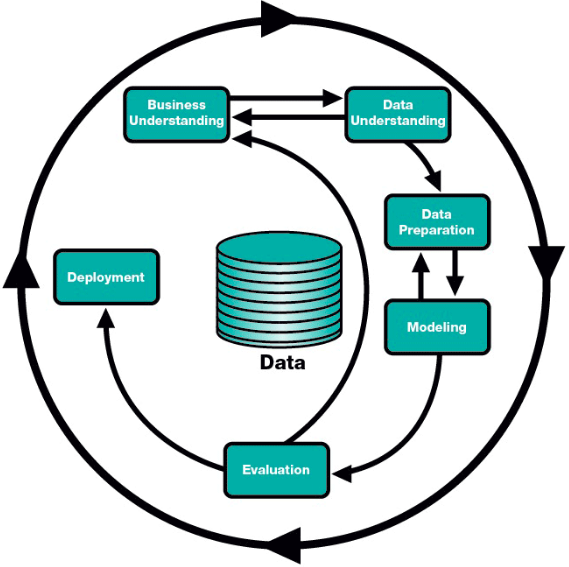
\includegraphics[scale=0.5]{img/crisp.png}
\captionof{figure}{\ac{crisp} Phasen \parencite{SmartVisionEurop}}\label{fig:crisp}
\end{center}
\textbf{Business Understanding}: diese Phase beschäftigt sich mit der Frage nach dem Ziel der Analyse. Dementsprechend, werden die Aufgaben erstellt und ein Plan festgelegt.\\
\textbf{Data Understanding}: die zweite Phase zielt darauf ab Daten zu sammeln und durch ein erstes Screening, deren Qualität festzustellen. Wie die Grafik \ref{fig:crisp} zeigt, kann dies dazu führen, die Ergebnisse aus der ersten Phase noch einmal anzupassen.\\ 
\textbf{Data Preparation}: nachdem Daten gesammelt wurden, gilt es anschließend diese für Analysen auf zubereiten. Hierbei liegt der Fokus darauf, die bestmögliche Konstruktion des finalen Datensatzes für die anschließende Modellierung zu gewinnen. Dazu ist es nötig relevante Daten auszuwählen und die Daten zu bereinigen. Dazu gehört sowohl das Entfernen und Korrigieren von Datenfehlern, als auch das Schätzen fehlender Daten durch Interpolation beispielsweise.\\
\textbf{Modeling}: diese Phase beschäftigt sich mit der Auswahl einer adäquaten Modellierungstechnik, wie zum Beispiel der Verwendung eines Decision Trees oder eines Neuronalen Netzes. Dazu gehört das kreieren eines Test- und eines Trainingsdatensets, womit verschiedene Modelle getestet werden können. Gegebenenfalls bedarf dies dem Wiederholen der Datenvorbereitung, um ein Datenset nochmals zu justieren.\\
\textbf{Evaluation}: währende dieser Phase wird das Modell welches die in Phase eins definierten Ziele am besten erfüllt, ausgewählt.\\
\textbf{Deployment}: in der letzten Phase werden die Ergebnisse aufbereitet und präsentiert und zusätzlich in einem Dokument festgehalten \parencite{SmartVisionEurop}.\\\\
Dieses Vorgehensmodell wurde für diese Arbeit ausgewählt, da es ein strukturiertes Vorgehen ermöglicht und dadurch die Qualität der Ergebnisse gesteigert werden kann. Das \emph{Business Understanding} besteht in dieser Arbeit darin, herauszufinden, was der momentane Stand der Forschung bezüglich Machine Learnning im Bereich Cyber Security ist. Anschließend werden bestehende Datensets untersucht, die der späteren Analyse dienen.
Um diese Daten anwenden zu können werden diese zunächst in der \emph{Data Preparation} Phase entsprechend aufbereitet. In der nächsten Phase, dem \emph{Modelling} werden diverse Algorithmen auf deren Passgenauigkeit überprüft. Anschließend wird der Algorithmus, welcher die Anforderungen am besten erfüllt, implementiert. Darüber hinaus wird das ganze Vorgehen ausführlich dokumentiert.

F-measure, Precision, Recall
\chapter{IOC - Bösartiges Verhalten}\label{sec:ioc}
Die permanente Steigerung in Größe und Komplexität von Computersystemen, bietet nicht nur einen höheren Nutzen für Kunden, sondern auch mehr Angriffsfläche für Hacker. Dies erschwert die Arbeit von Sicherheitsexperten. Da es darum geht die Kompromittierung eines Systems so früh wie möglich zu erkennen, um potenziellen Schaden zu verhindern, beziehungsweise diesen so gering wie möglich zu halten, arbeiten Experten gegen die Zeit.\\
Wurde ein System Opfer eines Angriffs, gilt es dieses forensisch zu untersuchen. Normalerweise hinterlässt ein Angreifer Spuren seines Einbruchs. Die Aufgabe der IT-Security ist es, diese zu finden. Diese Hinterlassenschaften werden als \emph{\acf{ioc}} bezeichnet, also Indikatoren, welche darauf hindeuten, dass ein System kompromittiert wurde.\\
%
\ac{iocs} müssen jedoch differenziert betrachtet werden. Es gibt eindeutige Indikatoren, welche kaum einen Zweifel daran lassen, dass ein System kompromittiert wurde. Angenommen ein Sicherheitsexperte findet Schadsoftware auf einem System und stellt gleichzeitig fest, dass es zu einem Datenupload auf einen nicht identifizierbaren Server kam, welcher von der Malware initiiert wurde. In diesem Fall kann davon ausgegangen werden, dass das System tatsächlich kompromittiert wurde. Der Indikator bildet sich hierbei aus den beiden Indizien: Malware und unautorisierter Upload.\\
Des Weiteren gibt es Indikatoren welche nicht eindeutig sind. Dieses Phänomen verdeutlicht das folgende Beispiel: angenommen, auf einer Maschine werden Prozesse erkannt, welche nicht von dieser selbst gestartet wurden, sondern durch remote gesendete Befehle. Diese können durch das Windows Tool \texttt{PsExec} übermittelt worden sein. Mit Hilfe dessen, lassen sich administrative Tätigkeiten, wie beispielsweise Systemupdates oder Passwort Änderungen, anhand von Remote-Befehlen durchführen. So vorteilhaft dieses Tool in den richtigen Händen erscheint, so gefährlich ist es in den falschen. Angreifer können \texttt{PsExec} für bösartige Zwecke missbrauchen. Zwar verlangt der Remote-Zugriff eine IP-Adresse mit korrespondierenden Benutzerinformationen, diese können jedoch durch andere Arten von Angriffen beschaffen werden. Da es sich bei \texttt{PsExec} um ein legitimiertes Tool zur Systemkoordination handelt, wird es von Anti-Viren Programmen nicht erkannt. Dadurch wird die Entdeckung eines Missbrauchs deutlich erschwert. Da die Benutzerinformationen allerdings unverschlüsselt übertragen werden, können immerhin diese über Tools wie \texttt{Wireshark} oder \texttt{Tcpdump} abgefangen werden. Der Nachweis über die Nutzung dieses Tools allein reicht also nicht aus, um eine Kompromittierung annehmen zu können.
\\\\
Bei der Malware spezifischen Analyse gilt es zunächst herauszufinden, was genau passiert ist und welches Schadprogramm für den Angriff verantwortlich ist. Traditionelle Anti-Virus Programme arbeiten basierend auf Datenbanken, in welchen sie bereits bekannte Signaturen und Heuristiken anwenden, um Malware zu identifizieren. Das Problem hierbei ist, dass es für Angreifer ein leichtes ist, ihren Code zu modifizieren, um die Signatur zu verändern, wodurch das Schadprogramm nicht mehr als solches erkannt wird. Verschleierungstaktiken wie diese, lassen sich in drei Gruppen einteilen \parencite{he2017model}:
\begin{itemize}
\item \textbf{Packing} Dies Bezeichnet die Technik exekutierbare Dateien zu komprimieren. Um die komprimierte Malware zu erkennen muss diese zunächst entpackt werden. Gleichzeitig ist dies aber auch ein guter \ac{ioc}, da ausführbare Dateien im Regelfall nicht komprimiert vorliegen.
\item \textbf{Metamorphismus} Hierbei wird die Erkennung erschwert in dem der Binärcode mutiert wird. Das bedeutet, die Sequenz der Opcodes wird bei jeder Ausführung geändert.
\item \textbf{Polymorphismus} Eine polymorphe Schadsoftware generiert bei jeder Ausführung eine weitere Version der Malware, sodass eine große Anzahl an divergierender Signaturen für dasselbe Programm entstehen.
\end{itemize}
Diese Techniken erschweren das Erkennen von Malware anhand gängiger Anti-Virus Programme deutlich. Zukünftig kann Machine Learning hierbei eine große Rolle spielen. Denn wie \textcite{Han2019} bereits erfolgreich untersuchten, ist auf \ac{mlas} basierende Erkennungssoftware in der Lage, Malware trotz dieser Verschleierungstechniken zu konstatieren.
\\\\
Das Erkennen von Malware basiert im Regelfall auf der Untersuchung von \ac{pes}. Diese beinhalten ausführbare Daten im Binärformat. Dazu gehören Windows \texttt{.exe} Dateien, Objektcode und \ac{dlls}. Eine \acs{pe} ist folgendermaßen aufgebaut:
\begin{center}
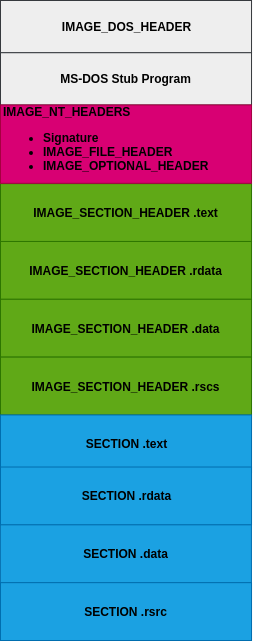
\includegraphics[scale=0.5]{img/pe.png}
\captionof{figure}{Aufbau einer \acs{pe} (eigene Darstellung)}\label{fig:pe}
\end{center}
Die in Abbildung \ref{fig:pe} grau hinterlegten Bereiche sind für die Analyse von \ac{pes} irrelevant, sie dienen unter anderem lediglich dazu, eine Fehlermeldung auszugeben, falls eine \texttt{.exe} Datei in einem Betriebssystem ausgeführt werden soll, mit welchem diese nicht kompatibel ist.\\
Der Bereich \texttt{IMAGE\_NT\_HEADERS} bietet bereits Informationen für eine Analyse. \texttt{IMAGE\_FILE\_HEADER} beinhaltet grundlegende Informationen bezüglich der Datei. Beispielsweise wann diese ausgeführt wurde, was einer Analyse sehr nützlich sein kann. Der Sektor \texttt{IMAGE\_OPTIONAL\_HEADER} ist entgegen dem was der Name vermuten lässt nicht \emph{optional}. Hier werden wichtige Informationen wie der Programmeinstiegspunkt, die Stackgröße zu Beginn sowie die Verwendung eines \ac{gui} (dt. \emph{Grafische Benutzeroberfläche}) oder einer Konsole definiert.\\
Die grün hinterlegten \texttt{IMAGE\_SECTION\_HEADER} bieten die interessantesten Informationen für eine Analyse. Diese \emph{Header} werden vom Compiler generiert und benannt, sodass der Benutzer wenig Kontrolle über die Namen hat. Dementsprechend konsistent ist die Benennung im Regelfall. Im PE-Header finden sich also relevante Informationen wie Imports, Exports, die Namen der verschiedenen Bereiche (blau hinterlegt), sowie deren Speichergröße auf der Festplatte und im \ac{ram}, sowie die Ressourcen welche von einem Programm benötigt werden.
\\\\
Grundsätzlich gibt es zwei Methoden um eine Malware Analyse durchzuführen: eine statische und eine dynamische.\\
Die Dynamische Analyse beinhaltet das Ausführen Schadhafter Programme. Dabei wird Malware in einer sicheren Umgebung ausgeführt und so dessen Verhalten analysiert. Dadurch kann im Gegensatz zur statischen Analyse die tatsächliche Verhaltensweise einer Datei untersucht werden, denn nicht jeder String der in einer Binärdatei gefunden wird, muss zwangsläufig ausgeführt werden. Des Weiteren können Logdateien analysiert werden, welche erst durch das Ausführen eines Programms entstehen.
Dynamische Analysen werden im Regelfall in einer \emph{Sandbox}, also in einem isolierten Bereich durchgeführt, wodurch kein Schaden an der Umgebung genommen wird.
Der Nachteil dieser Analyse besteht darin, dass die Malware die virtuelle Umgebung erkennen kann und sich somit stoppt. Des Weiteren können von der Schadsoftware benötigte Registry Keys oder Dateien in der virtuellen Umgebung fehlen, sodass deren Verhalten nicht korrekt aufgezeichnet werden kann.\\\\
Eine weitere Methode zur Malware Untersuchung bietet eine statische Analyse. Hierbei werden \ac{pes} erforscht. Zunächst durchläuft potenzielle Malware diverse Virenscanner, um die Entdeckung einer bösartigen Signatur zu erhöhen.\\ 
Des Weiteren kann \emph{Hashing} zum Einsatz kommen. Dabei wird ein eindeutiger \emph{hash} generiert, welcher verwendet werden kann, um zu recherchieren, ob dieser bereits von anderen AV-Dienstleistern analysiert wurde. Hashing bietet zudem den Vorteil, dass die Datei selbst noch nicht geteilt werden muss. Des Weiteren ist der Austausch eines Hashes auch um einiges schneller als der Upload einer Datei.\\
Programme verwenden Strings beispielsweise um sich mit einer URL verbinden zu können oder um Textausgaben zu drucken. Diese können einen guten Einblick über das Verhalten einzelner Programme liefern. Beispielsweise können dadurch IP Adressen für \ac{c2}-Systeme identifiziert werden, welche von Angreifern zum Verwalten von Remotesitzungen von infizierten Hosts verwendet werden.\\
Handelt es sich bei Dateien um sogenannte \emph{Packer}, also komprimierte Programme, müssen diese zunächst entpackt werden, um eine erfolgreiche Analyse durchführen zu können. Bei Dateien die relativ wenige Strings enthalten, handelt es sich meist um Packer. Wie die nachfolgende Tabelle zeigt, bietet die statische Analyse eine Vielzahl an Indikatoren, welche darauf hinweisen können, dass es sich bei der untersuchten Datei um Schadsoftware handelt.
%%%%%%%%%Table
\begin{table}[H]
\hspace{-2.8cm}
\begin{tabular}{lll}
\hline
\textbf{Ort} & \textbf{Indikator} & \textbf{Verhalten} \\ \hline
System & \begin{tabular}[c]{@{}l@{}}neue/modifizierte \\ Dateien\end{tabular} & Veränderung des Dateisystems durch Malware \\ \hline
System & Registry Einträge & Veränderung/Erstellung von Registry Keys \\ \hline
PE Header & wenige Imports & \begin{tabular}[c]{@{}l@{}}durch Packer komprimierte Dateien,\\ um die Erkennung und Analyse zu erschweren\end{tabular} \\ \hline
PE Header - Imports & \texttt{SetWindowsHookEx} & empfängt Tastatureingaben (Keylogger) \\ \hline
PE Header - Imports & \texttt{RegisterHotKey} & \begin{tabular}[c]{@{}l@{}}bestimmte Tastenkombination \\ startet Anwendung (Keylogger)\end{tabular} \\ \hline
IMAGE\_FILE\_HEADER & Kompilierungszeit & unsinnige Kompilierungszeit ist verdächtig \\ \hline
Sections & Abweichende Namen & z.B. .srtsa anstatt .data \\ \hline
SECTION .text & \begin{tabular}[c]{@{}l@{}}divergierende Speichergröße\\ von Virtual Size und Raw Size\end{tabular} & Packer extrahiert Code nach .text \\ \hline
SECTION .rsrc & eingebettetes Programm, Treiber & weitere durch Malware gestartete Aktionen \\ \hline
\end{tabular}
\caption{Auszug an, durch statische Analysen identifizierte Indikatoren für einen Malware Angriff (In Anlehnung an \textcite{Sikorski2012})}\label{table:pe}
Diese Indikatoren aus Tabelle \ref{table:pe}, sind nur ein kleiner Teil dessen, was bei einer statischen Analyse entdeckt werden kann. Dennoch wird dadurch deutlich, wie hilfreich \ac{pes} im Erkennen von Malware sein können.\\ 
Welche Features aus diesen Dateien generiert werden können, um eine aussagekräftige Untersuchung mit Hilfe von \ac{mlas} zu generieren, wird in diversen Ansätzen beschrieben, mit welchen sich das folgende Kapitel beschäftigt.
%%%%%%%%%%%%%Table
\label{tab:iocs}
\end{table}
\chapter{Analyseverfahren}
\label{sec:ba}
%\section{Machine Learning - Evaluationskriterien}
%\label{sec:mle}
Das folgende Kapitel beschäftigt sich mit Machine Learning Verfahren, welche für die Erkennung von Cyber Security Angriffen verwendet werden. Diese Verfahren wurden anhand einer umfangreichen Literaturrecherche ermittelt. Jedes Vorgehen wird auf dessen verwendete Algorithmen sowie der ausgewählten Features untersucht. Des Weiteren wird analysiert welche Evaluationskriterien verwendet wurden um die Effektivität zu messen und zu welchem Ergebnis der jeweilige Ansatz führte.\\
Das Vorgehen hierbei, orientiert sich an einem problembezogenen Ansatz. Dazu wird im Folgenden eine Übersicht darüber generiert, welche Probleme aus der Cyber Security bereits von Machine Learning Algorithmen in Angriff genommen wurden. Dies dient einer übersichtlichen Darstellung der Möglichkeiten und zeigt die Diversität auf, in welcher \ac{mlas} die Arbeit von Cyber Security Spezialisten unterstützen und verbessern können.\\\\
Zunächst werden Verfahren erläutert, welche bereits wissenschaftlich belegt wurden. Wurden, dem Ansatz entsprechende Adaptionen aus der Industrie identifiziert, wurde der jeweilige Ansatz um den industriellen erweitert.
%\section{Ansätze aus der Wissenschaft}
%\label{sec:aw}
%Das Einsatzgebiet von Machine Learning Algorithmen im Kontext von Cyber Security ist sehr breit gesteckt und reicht von der Untersuchung von Spam Profilen bei Twitter, über die Klassifizierung von Netzwerkverkehr bis hin zur Erkennung böswilliger SQL-Abfragen. Die Untersuchung dieses breit gefächerten Spektrums würde den vorgesehenen Umfang dieser Arbeit deutlich überschreiten. Infolgedessen werden lediglich Analysen dokumentiert, welche sich mit der Erkennung und Klassifizierung von Malware beschäftigen.


Für die Recherche wurden alle Verfahren in einem Zeitraum von 2015 bis heute berücksichtigt. Diese Periode wurde gewählt, da sich die Zahl der Cyberangriffe, sowie die zur Verfügung stehende Schadsoftware bereits innerhalb weniger Jahre deutlich vermehrt beziehungsweise verändert. Somit soll verhindert werden veraltete Angriffsvektoren zu analysieren, welche bereits von moderneren überholt wurden. Zusätzlich gibt es bereits vergleichbare Arbeiten aus dem Jahr 2016 \parencite[s.][]{Buczak2016}, in welchem Machine Learning Ansätze vor dieser Zeit analysiert werden.\\
In der folgenden Auflistung wird die Bezeichnung \glqq Erkennung\grqq für binäre Klassifikation verwendet. Beispielsweise, wenn sich ein Ansatz darauf beschränkt Daten entweder in die Rubrik A \glqq bösartig\grqq oder in die Rubrik B \glqq gutartig\grqq zu klassifizieren.\\
Erfolgt in einem Analyseverfahren eine Einteilung in mehrere Klassen (mehr als zwei), wird nachfolgend der Begriff 
\glqq Klassifizierung\grqq verwendet.
\\\\
%%%%%%%%%%%%%%%%%%%%%%%%%%%%%%%%%%%%%%%%%%%%%%%%%%%%%%%%%%%%%%%%%%%%%%%%%%%%%%
%wenn binäre Klassifikation:
%%%%"Erkennung von..."
%Wenn Multiclass Klassifizierung:
%%%%"Klassifizierung von..."
%Ansonsten "..Erkennung" etc.
%%%%%%%%%%%%%%%%%%%%%%%%%%%%%%%%%%%%%%%%%%%%%%%%%%%%%%%%%%%%%%%%%%%%%%%%%%%%%%
\section{Erkennung von Malware - Hybride Analyse (2015)}
Im Jahr \citeyear{Shijo2015} haben \citeauthor{Shijo2015} einen, auf zwei Analysen basierenden, Ansatz gewählt, um Malware zu erkennen. Zum einen verwendeten sie ein statisches Analyseverfahren bei dem sie \emph{Printable Strings}, also nicht kodierte Zeichenfolgen wie z. B. \emph{FindFirstFile} aus Binärdateien extrahierten. Zum anderen konfigurierten sie eine Cuckoo Sandbox, in der sie Schadsoftware ausführten und deren API Aufrufe in einer Logdatei speicherten.\\
Sie untersuchten die Ähnlichkeit in API-Aufrufsequenzen anhand von n-Gramm-basierter Ähnlichkeitsmessung. 
Als Features dienten Tri- und Tetragramme ab einer gewissen Häufigkeit, sowie PrintableStrings ab einer Häufigkeit von zwei.
Für die Klassifizierung wurden die Algorithmen \ac{rf} und \ac{svm} verwendet.
Es wurden jeweils beide Ansätze separat, sowie in Kombination getestet. Analysen mit \ac{svm} erzielten eine Genauigkeit von 95.88 \% für die statische Analyse und 97.16 \% für die dynamische Analyse und waren somit erfolgreicher, als Untersuchungen mit Random Forest. Die besten Ergebnisse erzielte der hybride Ansatz mit \ac{svm} mit einer Genauigkeit von 98.71 \% und der geringsten \ac{fpr} von 0.026.\\
Die Forschung von \citeauthor{Shijo2015} zeigt also, dass mit den von ihnen gewählte Features, mit einem hybriden Ansatz, deutlich genauere Aussagen, als mit rein statischen oder rein dynamischen Analysen, getroffen werden können.

%
\section{Erkennung von Malware - Statische Analyse (2016)}
\citeauthor{More2016} untersuchten EXE-Dateien auf Schadsoftware. Dazu konvertierten sie die Dateien zunächst in \ac{opcode}, also in den Teil der Maschinensprachanweisung der die auszuführenden Operationen angibt, z.B. \texttt{55 8B EC 83 EC 5C 83 7D 0C 0F 74 2B 83 7D 0C 46}. Das ausgewählte Feature Datenset wurde anschließend nochmals zu einer \ac{arff} Datei konvertiert, um die Datei nachfolgend mit der Machine Learning Software Weka bearbeiten zu können. 
In Weka wurden die Algorithmen JRip, C4.5 und IBk verwendet. Wobei es sich bei JRip und C4.5 um \ac{dt} und bei IBk um \ac{knn} Implementierungen handelt. Um die Erkennungsgenauigkeit zu erhöhen, wurden nicht die einzelnen Algorithmen, sondern ein Klassifikatorensemble angewandt, um Methoden wie Mehrheitsvoting, Veto-Voting und vertrauensbasiertes Veto-Voting verwenden zu können. Ersteres folgt demokratischen Regeln, das heißt, die Klasse mit den meisten Stimmen ist das Ergebnis. Veto-Voting hingehen basiert auf Annahmen über die Wahl der anderen Algorithmen. Vertrauensbasiertes Veto-Voting ergänzt voriges Voting um eine Vertrauensberechnung, wodurch jedem Algorithmus ein bestimmtes Vertrauensniveau zugeteilt wird. \\
\citeauthor{More2016} konnten zeigen, dass durch die Verwendung von Veto-Voting eine Genauigkeit von 80.7 \% erzielt werden kann. Im Vergleich dazu, lag das beste Ergebnis, welches durch singulären Algorithmeneinsatz von IBk erzielt wurde, bei einer Genauigkeit von nur 73.5 \%.\\\\
Dieses Ergebnis stützt die These von \citeauthor{Shijo2015} aus dem Jahr zuvor, welche zeigten, dass ein nicht-hybrider Ansatz weniger genau ist, als einer, der die statische und die dynamische miteinander verknüpft.
\section{Erkennung bösartiger XML-basierter Office Dokumente(2016)}
Durch das neue Dateiformat, welches Microsoft 2007 auf den Markt gebracht hat, sollten Sicherheitslücken geschlossen werden.
Das Binärformat wurde durch ein	XML basiertes Dateiformat ersetzt. Dadurch werden neue digitale Funktionen unterstützt, sowie vertrauensbasierte Bereiche geschaffen, welche das Format weniger riskikoreich gestalten sollen. Nichtsdestotrotz können Attacken gegen XML-basierte Office Dokumente gestartet werden. Zu den möglichen Angriffsvektoren zählen beispielsweise macrobasierte Attacken. Durch den Missbrauch von \ac{vba} kann die zugehörige shell gestartet werden, um willkürliche Kommandos zu senden. Außerdem können externe Bibliotheken sowie Programme aufgerufen werden, welche Schaden verursachen können. Eine weitere Bedrohung durch den Gebrauch von Macros bildet die Fähigkeit dieser, bösartige Dateien aus dem Internet herunterzuladen.\\
\textcite{Cohen2016} haben in ihrer Arbeit diese Art von Attackvektoren untersucht, um eine Infizierung durch bösartige Macros frühzeitig zu erkennen. Dazu haben sie zunächst Office Dokumente in eine Liste von Pfaden konvertiert. Diese dienen der Analyse als Features. Dadurch wurde jedoch eine so hohe Anzahl an Features generiert, dass die Untersuchung mit verschiedenen Datensets durchgeführt wurde, welche Top Features von 10 bis 2000 beinhalteten. Um die Feature-Repräsentation, also das Vorhandensein bzw. die Wichtigkeit von Features zu bestimmen, wurden zwei Verfahren angewandt. Zum einen ein binäres Verfahren, welches lediglich die Ab-, respektive Anwesenheit eines Features misst und zum anderen wurde das statistische Verfahren \ac{tfidf} verwendet, um die Wichtigkeit eines Terms in Bezug auf ein Dokument zu bestimmen. Anschließend wurden die Daten mit folgenden Algorithmen untersucht: J48, \ac{rf}, \ac{lr}, \ac{nb}, \ac{bn}, \ac{lb}, \ac{smo}, Bagging und \ac{ab}. \\\\
Wie die Ergebnisse zeigen, erzielt das Datenset mit den Top 200 Features, welches mit Random Forest analysiert wurde die besten Werte mit einem F-measure von 0.66.
Wie sich demonstrieren ließ, ist es möglich bösartige Office Dokumente durch eine Analyse deren Pfade zu erkennen. 
Die Untersuchung beschränkt sich jedoch auf direkte Gefahren innerhalb von Dokumenten. Indirekte Gefahren, wie etwa die durch weiterführende Links, wurden in dieser Forschungsarbeit nicht berücksichtigt.
\section{Erkennung bösartiger HTTP-Anfragen (2016)}
\textcite{Pham2016} haben in ihrer Arbeit ein \ac{ids} für \ac{http} - Anfragen entwickelt. Dazu nutzen sie ein von ihnen entwickeltes Modul, um Netzwerkpakete zu erfassen. Dieses Modul basiert auf derselben Erfassungstechnik die \texttt{Wireshark} verwendet. Um ein geeignetes Model zu zu evaluieren, welches es ermöglicht die Pakete in Echtzeit zu klassifizieren, wurden diverse \ac{mlas} anhand des CSIC 2010 HTTP Datensets von \textcite{csic} getestet. Dieses besteht aus 223585 Daten die entweder als \emph{normal} oder \emph{anomal} beschriftet sind. Es enthält Attacken wie SQL-Injections, Buffer Overflow und \ac{xss}. \citeauthor{Pham2016} trainierten und testeten die Daten mit den Algorithmen Decision Tree, Random Forest, AdaBoost, Logistic Regression und dem  SGDClassifier. Als Evaluationsmethode wurden Precision, Recall und F-measure verwendet. Den höchsten dieser Werte erzielte die Logistic Regression Methode mit einem F1-measure von 96.11 for abnormen und 95.82 für normalen Verkehr. Zukünftig sollen diese Ergebnisse an Paketen, welche durch das eigens entwickelte Modul der Forscher erfasst wurden, evaluiert werden.
%
\section{Klassifizierung von Netzwerkattacken (2017)}
\textcite{Yin2017} implementierten ein \ac{ids}, für welches sie \ac{rnns} verwendeten. Zusätzlich wurde die Leistung des Models bei binärer als auch bei Multi-Klassen Klassifikation untersucht. Um die Effizienz zu prüfen, wurde ferner ein Vergleich mit diversen \ac{mlas} gezogen. Die Analyse basiert auf dem NSL-KDD Datenset aus dem Jahr 2009. Dieses beinhaltet neben dem normalen Netzwerkverkehr, Daten zu vier verschiedenen Angriffstypen die da wären: \ac{dos}, \ac{r2l}, \ac{u2r} und Probe Attacken. Das Datenset besteht aus 41 Features. Um Vergleiche mit anderen \ac{mlas} herzustellen, wurden parallel Experimente mit \ac{ann}, \ac{rf}, \ac{nb}, \ac{mlp}, \ac{svm}, J48, Random Tree und \ac{nbt} für die binäre Klassifikation durchgeführt. Auf dieselbe Weise wurde die Multi-Klassen Klassifikation überprüft. Als Qualitätsmerkmal der Ergebnisse wurde der Wert \emph{Accuracy} gewählt, welcher die Genauigkeit der Analyse wider spiegelt. Dieser Wert basiert auf dem Prozentsatz der korrekt klassifizierten Daten im Vergleich zur Gesamtheit der Daten. Das Ergebnis zeigt, dass \ac{rnns} eine qualitativ hochwertigere Analyse produzieren als die zu verglichenen \ac{mlas}. Bei der binären Klassifikation des Testsets erzielte auf \ac{rnns} basierende Untersuchungen eine Genauigkeit von 83.28\% gefolgt von \ac{nbt} mit 82.02\%. Bei der Klassifizierung in fünf Klassen erreichte das \ac{rnn} mit 81.29\% ebenfalls ein besseres Ergebnis als die restlichen Algorithmen. Jedoch fanden \citeauthor{Yin2017} heraus, dass \ac{rnns} deutlich mehr Zeit für das Training beanspruchen, dieses Problem soll zukünftig durch Beschleunigung der \ac{gpu} behoben werden.
%
\section{Erkennung von Ransomware - Dynamische Analyse (2017)}
\citeauthor{Maniath2018} haben eine dynamische Analyse entwickelt um \emph{Ransomware} anhand von API Aufrufen zu klassifizieren. Ransomware beschreibt eine Art Schadprogramm, welche dem Benutzer Ressourcen entzieht und eine Lösegeldsumme verlangt um diese wieder verfügbar zu machen. Um die Aufrufe zu extrahieren verwendeten die Forscher die dafür entwickelte Umgebung von Cuckoo Sandbox. Dadurch konnten die Schadprogramme in einer Umgebung ausgeführt werden ohne Schaden zu erzeugen. Die Anwendung erfasst alle API Aufrufe und speichert diese in einer \texttt{.json} Datei. Für die Analyse wurden 157 schadhafte Dateien aus nicht näher beschriebenen Onlinequellen verwendet. Dabei konnten 239 Aufrufe extrahiert werden, welche der Untersuchung als Features dienten. Um eine einheitiche Länge dieser zu gewährleisten, wurden die einzelnen Aufrufe entsprechend der längsten Sequenz mit Nullen aufgefüllt. Anschließend wurden die Daten entweder mit 0 für \emph{gutartig} oder mit 1 für \emph{ransomware} etikettiert. Anhand dieser Daten wurde ein \ac{lstm} Netzwerk trainiert. Nach einer Trainingszeit von zwei Stunden erreichte das Model eine Genauigkeit von 96.67\% bei der Analyse der Testdaten. Die komplette Prozess einschließlich der Gewinnung der API Sequenzen dauerte allerdings 56 Stunden, was in anbetracht der geringen Menge an Datensätzen doch sehr nachteilig ist.
%
\section{Erkennung von Malware - Imageanalyse (2017)}
Eine potenziell schnellere Methode um Malware zu erkennen, entwickelten \citeauthor{8190895} anhand einer Image Analyse. Dazu generieren sie Bilder von ausführbaren Dateien. Dabei hat jedes Pixel einen Wert zwischen 0 und 255. Um aus einer Datei ein Bild zu erhalten, wird jedes Byte eingelesen und zu einer Ganzzahl konvertiert die einem Pixel entspricht. Dadurch entstehen 256x256 Bilder. Da dadurch während einer Analyse der Speicher zur Neige geht wurden die Daten auf 32x32 reduziert. Die dadurch generierten Bilder dienen der Analyse mit einem \ac{cnn} als Features. Die 2000 dafür verwendeten Schadprogramme, stammen aus einem koreanischen Cyber Security Forschungszentrum. Als Metrik zur Überprüfung der Genauigkeit wurde hier ebenfalls die Genauigkeit gewählt, welche sich auf 95.66\% beläuft.\\
Bedauerlicherweise haben \citeauthor{8190895} nicht erwähnt in welcher Geschwindgkeit sie ihre Analyse durchführen konnten. In Anbtracht der von ihnen aufgestellten These - Imageanalysen seien viel schneller als statische und dynamische Analysen - wäre dies ein interessantes Detail gewesen.

%
\section{Erkennung böswilliger MS Office Dateien (2017)}
\citeauthor{Bearden2018} konzentrierten sich in ihrer Forschung darauf eine Methode zu entwickeln, mit welcher sich Microsoft Office Dokumente anhand ihrer Macros nach \emph{gutartig} und \emph{bösartig} klasifizieren lassen. Dazu untersuchten sie 158 Dateien, von welchen 40 schadhaft waren. Dokumente die Macros enthalten, beinhalten nicht nur \ac{vba} Code sondern auch \emph{p-code}. Dabei handelt es sich um Assemler-Code, welcher vom \ac{vba}-Interpreter generiert wird, nachdem der Code einmal ausgeführt wurde \parencite{Bearden2018}. Diese Codes dienten der Analyse mit \ac{knn} als Features. Die Effizienz wurde, wie die beiden zuletzt erläuterten Ansätze, anhand der Genauigkeit gemessen. Es wurden verschiedene Experimente mit unterschiedlichen \emph{K} und \emph{L} durchgeführt, wobei \emph{K} die Anzahl an Clustern und \emph{L} die Anzahl der besten Features impliziert. Den besten Wert erzielte eine Kombination mit K=3 und den Top 75 Features mit einer Genauigkeit von 96.3\%.\\Es wurde auschließlich ein Algorithmus getestet, da die Intention der Forschung darin bestand , einen \emph{Proof of concept} für die Erkennung bösartiger Macros anhand von p-codes bereitzustellen. Der Vorteil den \citeauthor{Bearden2018} mit ihrer Forschung geschaffen haben, besteht darin, dass potenziell bösartige Dateien nicht geöffnet werden müssen, bevor sie analysiert werden können. Jedoch weisen auch sie auf den Mangel an adäquaten Trainingsdaten hin, welchen es zukünftig zu beheben gilt.
%
\section{Klassifizierung von \ac{ddos} Attacken (2017)}
Bereits seit den 80er jahren gibt es \ac{dos} Attacken, welche Netzwerk Ressourcen erschöpfen und dadurch die Verfügbarkeit von Services blockieren. Es gibt zwei Arten diese Attacken zu erkennen: Zielseitige Verteidigung und Quellenseitige Verteidigung\parencite{He2017}. Die Zielseitige Erkennung hat den Nachteil, dass Attacken erst entdeckt werden nachdem sie bereits beim Opfersystem ankamen. \citeauthor{He2017} forschen an einem proaktiven Ansatz, bei dem die Erkennung auf der Quellenseite erfolgen soll, wodurch Angriffe auf mehrere Systeme verhindert werden können. Dabei konzentrieren sie sich auf vier gängige \ac{ddos} Angriffe aus der Cloud: \ac{ssh} brute-force Attacken, \ac{icmp} flooding Attacken, \ac{dns} reflection Attacken und \ac{tcp} \ac{syn} Attacken. Als Feature für \ac{ssh} brute-force Attacken dient die Anzahl an Diffie-Hellman Schlüsselaustausche, da dieser Wert während einer solchen Attacke steigt \parencite{He2017}. Als Feature für \ac{dns} reflection Attacken wurde das Verhältnis von eingehenden und ausgehenden \ac{dns}-Paketen gewählt, da bei einer Attacke mehr Anfragen als Antworten gesendet werden. Die \ac{icmp} Paketrate wurde als Feature für \ac{icmp} flooding Attacken gewählt, da bei normalem Verkehr eine geringere Anzahl dieser Pakete vorhanden ist. Um ac{tcp} \ac{syn} Attacken zu identifizieren, wurde das \ac{syn}/\ac{ack} Verhältnis als Feature gewählt, da während einer solchen Attacke mehr \ac{syn} Tags als \ac{ack} Tags in den Paketen zu finden sind. Für das Experiment wurde der Netztwerkverkehr 9 Stunden lang verfolgt und anschließend mit den Algorithmen \ac{lr}, \ac{svm}, \ac{dt}, \ac{nb}, \ac{rf}, k-means und \ac{gmm} klassifiziert. Zur Evaluation dienten die Metriken: Precision, Genauigkeit, Recall und F1-measure. Das beste Ergebnis mit einem F1-measure von 0.9975 und einer Genauigkeit von 99.73\% konnte mit \ac{svm} erzielt werden.
Durch diesen vielversprechenden Ansatz sollen zukünftig weitere \ac{ddos} Attacken proaktiv erkannt werden.
%
\section{Schwachstellen Scanner für Web Applikationen (2017)}
\textcite{VidyavardhakaCollegeofEngineering2017}...
%
\section{Erkennung von Malware anhand von PE-Header (2017)}
\textcite{Raff2017}...
%
\section{Erkennung von Malware anhand von PE-Header mit erweitertem  Feature-Set (2017)}
\textcite{Kumar2017}...
%
\section{Erkennung von Exfiltration und \ac{cc}Tunnels (2017)}
\textcite{Das2018}...
%
\section{Erkennung bösartiger PowerShell-Befehle (2018)}
\textcite{Hendler2018}...
%
\section{Klassifizierung von Netzwerkverkehr in 5 Klassen (2018)}
\textcite{Ding2018}...
%
\section{Anomalieerkennung anhand von Systemprotokollen (2018)}
\textcite{Brown2018}...
%
\section{Erkennung von bösartigem Netzwerkverkehr (2018)}
\textcite{Aldwairi2018}...
%
\section{Erkennung von Botnetzen (2018)}
\textcite{Mathur2018}....
%
\section{Klassifizierung von Microsoft Malware (2018)}
\textcite{Sabar2018}....
%
\section{Klassifizierung von Malware anhand von Datenpaketen (2018)}
\textcite{Yeo2018}...
%
\section{Erkennung von Portscans (2018)}
\textcite{Aksu2019}
%
\section{Klassifizierung von Netzwerkverkehr in 3 Klassen (2018)}
\textcite{Teoh2018}...
%
\section{Erkennung bösartiger SQL-Abfragen (2018)}
\textcite{Jayaprakash2018}...
%
\section{Erkennung von \ac{lddos} Attacken (2018)}
\textcite{siracusano2018detection}...
%
\section{Klassifizierung von Wi-Fi Netzwerkdaten (2018)}
\textcite{Qin2018}....
%
%
\section{Klassifizierung von Malware anhand einer systematischen Profilerstellung (2019)}
\textcite{he2017model} Malware Verschleierung durch packing, Metamorphism und Polymorphism.\\
\textcite{Han2019}...\\
.....
Neueste Forschungen zeigen, dass dynamische und statische Analyseverfahren zu ungenau sind, um neue Schadsoftware in Echtzeit zu erkennen \parencite{Vinayakumar2019}. Dazu bedarf es Deep Learning Verfahren, wie der folgende Ansatz verdeutlicht.
%
\section{Klassifizierung von Malware - Imageanalyse (2019)}
Um Polymorphismus, Metamorphismus und Packing zu erkennen ist ein umfangreiches Feature Engineering, sowie beträchtliche Kenntnisse auf Domain-Ebene nötig \parencite{rhode2018early}. Zudem können Angreifer der automatischen Malware Erkennung entgehen sobald sie die verwendeten Features kennen \parencite{anderson2017evading}. Diesen Problemen wollen \textcite{Vinayakumar2019} mit ihrem Deep Learning Ansatz begegnen.\\
Dazu verglichen sie klassische Algorithmen für maschinelles Lernen mit Deep Learning Architekturen. Die Vergleiche basieren auf statischen und dynamischen Analysen, sowie auf Bildverarbeitungstechnologien.\\
...\\ 
Wie sich zeigte ist die Imageanalyse schneller als die statische und die dynamische Analyse, da diese auf Rohdaten basiert und komplett auf Zerlegung oder Ausführung von Code verzichtet.


\section{Erkennung von \ac{ff} Netzwerken (2019)}
\textcite{Chen2019}...
%
\section{Erkennung von drive-by Download-Attacken bei Twitter (2019)}
\textcite{Javed2019}...
Verschleierte Links können dazuführen dass der Angreifer Fernzugriff zum System des Opfers bekommt von welchem er Daten klauen kann oder dessen Computer in ein Botnetz integrieren kann \parencite{provos2007ghost}.
%
\section{Erkennung von \ac{dga} Domains (2019)}
\textcite{Li2019}...
%
\section{Erkennung von Phishing Websites (2019)}
Phishing zielt im Vergleich zu anderen Attacken nicht darauf ab Schwachstellen im System auszunutzen, sondern durch Sicherheitslücken beim Menschen an dessen sensitive Informationen wie Benutzernamen und Passwörter zu gelangen.
In der Forschung gibt es momentan vier Verfahren, um Phishing Websites zu erkennen:\\
Blacklists, Heuristiken, Inhaltsanalysen und Machinelles Lernen. Blacklists gleichen URLs mit bekannten Phishing Websites ab, Heuristiken verwenden Signaturdatenbanken bekannter Angriffe um sie mit der Signatur eines heuristischen Musters abzugleichen. Inhaltsanalysen versuchen Phishing Websites mit Hilfe bekannter Algorithmen wie \ac{tfidf} zu identifizieren. \\
Der im Folgende beschriebene Ansatz von \textcite{Alswailem2019} verwendet Machine Learning Verfahren, um Phishing Websites zu erkennen.
%
\section{Erkennung von Insider Bedrohungen (2019)}
\textcite{Le2019}...
%
\section{Erkennung von bösartigen PDFs (2019)}
\textcite{Jeong2019}...
%
%Next Section%%%%%%%%%%%%%%%%%%%%%%%%%%%%%%%%%%%%%%%%%%%%%%%%%%%%%%%%%%%%%%%%%%%%%%%%%%%%%%%%%%%%%%%%%%%%%%%%%%%%%%%%%%%%%%%%%%%%
%\section{Ansätze aus der Industrie}\label{sec:ai}
%\textcite{Microsoft2019}
\chapter{Datensätze}
\chapter{Prototypische Implementierung}
\chapter{Diskussion}
\chapter{Fazit}
\chapter{Zukünftige Forschung}
\newpage
\frontmatter 
\pagenumbering{Roman}
\appendix
%\renewcommand{\refname}{Literaturverzeichnis}
%\bibliographystyle{plaindin}
%\bibliography{Bibtex/Masterarbeit-ma}
\printbibheading[heading=bibnumbered]
%
% einfache Möglichkeit der Trennung von Quellenarten via keyword
%
\printbibliography[notkeyword=internet, heading=subbibliography, %
   title={Bücher und Journals}]
\printbibliography[keyword=internet, heading=subbibliography, %
   title={Internetquellen}]
\renewcommand{\listfigurename}{Abbildungsverzeichnis}
\listoffigures
\renewcommand{\listfigurename}{}
\listoftables
\chapter{Abkürzungsverzeichnis}
\addcontentsline{toc}{section}{\textbf{Abkürzungsverzeichnis}}
\begin{acronym}
\acro{ab}[AB]{AdaBoost}
\acro{ack}[ACK]{acknowledge}
\acro{ann}[ANN]{Artificial Neural Network}
\acro{apts}[APTs]{Advanced Persistent Threats}
\acro{arff}[ARFF]{Attribute-Relation File Format}
\acro{bitkom}[BITKOM]{ Bundesverband Informationswirtschaft,Telekommunikation und neue Medien e.V.}
\acro{bka}[BKA]{Bundeskriminalamt}
\acro{bn}[BN]{Bayesian Network}
\acro{cc}[C\&C]{Command \& Control}
\acro{cnn}[CNN]{Convolutional neural network}
\acro{crisp}[CRISP-DM]{Cross-industry standard process for data mining}
\acro{c2}[C2]{Command and Control}
\acro{dos}[DoS]{Denial of Service}
\acro{ddos}[DDoS]{Distributed Denial of Service}
\acro{dga}[DGA]{Domain Generation Algorithm}
\acro{dlls}[DLLs]{Dynamic Link Libraries}
\acro{dns}[DNS]{Domain Name System}
\acro{dt}[DT]{Decision Tree}
\acro{ff}[FF]{Fast-Flux}
\acro{fpr}[FPR]{False Positive Rate}
\acro{gmm}[GMM-EM]{Gaussian-Mixture Model for Expectation-Maximization}
\acro{gui}[GUI]{Graphical User Interface}
\acro{gpu}[GPU]{Graphics processing unit}
\acro{http}[HTTP]{Hypertext Transfer Protocol}
\acro{icmp}[ICMP]{Internet Control Message Protocol}
\acro{ids}[IDS]{Intrusion Detection System}
\acro{ioc}[IoC]{Indicator of Compromise}
\acro{iocs}[IoCs]{Indicators of Compromise}
\acro{knn}[k-NN]{k-nearest-neighbor}
\acro{lb}[LB]{LogitBoost}
\acro{lddos}[LDDoS]{Low-rate DDoS}
\acro{lr}[LR]{Logistic Regression}
\acro{lstm}[LSTM]{Long-Short Term Memory}
\acro{mlas}[MLAs]{Machine Learning Algorithmen}
\acro{mlp}[MLP]{Multi-Layer Perceptron}
\acro{nb}[NB]{Na\"ive Bayes}
\acro{nbt}[NBTree]{Na\"ive Bayesian Tree}
\acro{opcode}[Opcode]{Operation Code}
\acro{pe}[PE-Datei]{Portable Executable Datei}
\acro{pes}[PE-Dateien]{Portable Executable Dateien}
\acro{psi}[PSI]{Printable String Information}
\acro{ram}[RAM]{Random-Access Memory}
\acro{rnn}[RNN]{Recurrent neural network}
\acro{rnns}[RNNs]{Recurrent neural networks}
\acro{rf}[RF]{Random Forest}
\acro{rnnids}[RNN-IDS]{Rekurrente neuronale Netze für Intrusion Detection Systems}
\acro{r2l}[R2L]{Remote to Local}
\acro{smo}[SMO]{Sequential Minimal Optimization}
\acro{ssh}[SSH]{Secure Shell}
\acro{svm}[SVM]{Support Vector Machine}
\acro{syn}[SYN]{synchronize}
\acro{tcp}[TCP]{Transmission Control Protocol}
\acro{tfidf}[TF-IDF]{Term Frequency - Inverse Document Frequency}
\acro{tpr}[TPR]{True Positive Rate}
\acro{u2r}[U2R]{User to Root}
\acro{vba}[VBA]{Visual Basic for Applications}
\acro{xss}[xss]{Cross-site scripting}

\end{acronym}
%\end{document}
\newpage

\chapter{Anlagen}
\addcontentsline{toc}{section}{Anlagen}
\subsection*{Anlage 1: Research Model}\label{rm}

\begin{figure}[h!]
\hspace{-2.3cm}
%\begin{center}
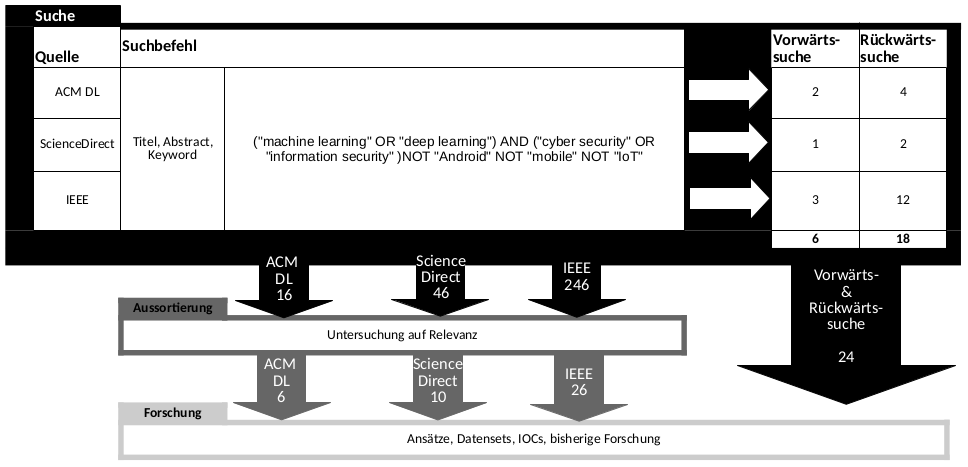
\includegraphics[width=1.3\textwidth]{img/rm}
\caption*{Prozess der Literaturrecherche}
%\end{center}
\end{figure}
\newpage
\subsection*{Anlage 2: Literaturreview}\label{literaturr}

\begin{figure}[h!]
\hspace{-2.2cm}
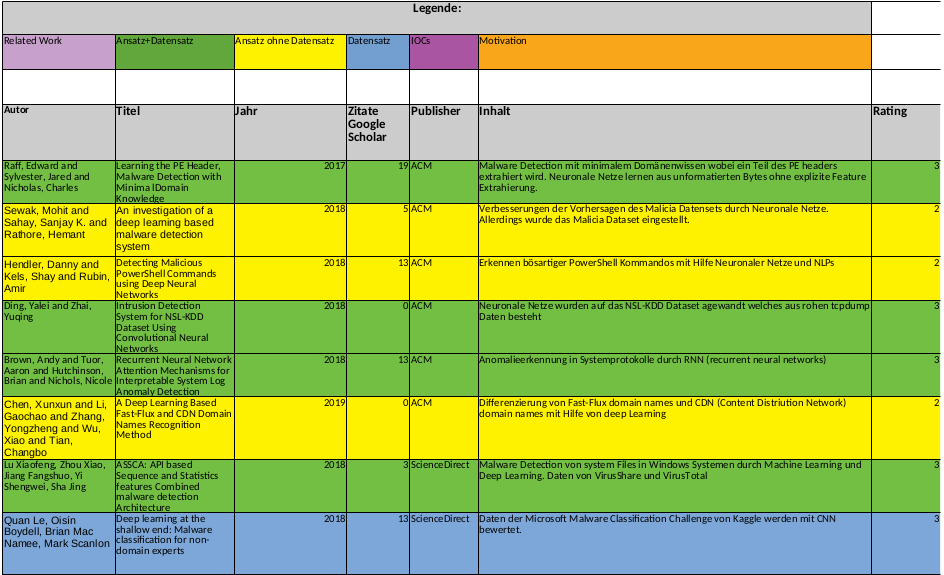
\includegraphics[width=1.3\textwidth]{img/literaturr}
\caption*{Ausschnitt der Literaturreview Liste}
\end{figure}
\end{document}